\scanpage{21}
Orientation d'une \uline{arête} : par choix d'une ``origine''.
% slanted
\margin{Orientations opposées}
Orientation induite sur le bord de l'arête (extrémité -- origine)

Orientation d'un contour combinatoire : choix d'une orientation sur chaque arête, de telle façon que pour tt sommet $s$, les deux orientations induites sur $s$ soient opposées
\diagram{\begin{tikzcd}[ampersand replacement=\&,row sep=.2em,column sep=2em]
{} \arrow[dr] \& \& {}\\
\& \bullet \arrow[ur] \&
\end{tikzcd}}

\deleted{\unsure{Rem}} Relations avec le cas topologique ; orientation d'un segment topologique, d'une $1$-variété topologique

\uline{Théorème} a) Tout \uline{\unsure{polygône|polygone}} combinatoire admet \unsure{exactemt|exactement} $2$ orientations, \unsure{opposées} \deleted{\unsure{l'une à l'autre}} l'une de l'autre.
% slanted
\margin{S'il y a $r$ comp. connexes, alors il y a $2^r$ orientations}

b) À toute orientation $\omega$ \inserted{d'un contour,} correspond un unique \unsure{autom|bijection} $\rho_\omega$ tel que

1) $\rho_\omega$ conserve l'orientation

2) $\forall s\in S$, $\deleted{\unsure{\rho}}(s,\rho_\omega(s))$ soit une \uline{arête} $\underline a$, dont l'origine $o_\omega(a)$ soit $s$.
% slanted
\margin{\unsure{$\alpha$)|2)|b)} $\forall s\in S$, $\deleted{\unsure{\rho}}\rho(s)$ est adjacent à $s$\\
\unsure{$\beta$)|3)} $\forall a\in A$, $\rho(a)$ est adj. à $a$ \quad NB\\
$\alpha$) et $\beta$) sont \unsure{équivalents|équivalentes}, s'il n'y a pas de comp. bigone}

\deleted{c) $\omega\mapsto\rho_\omega$ est une \unsure{corr.|corresp.} $1$-$1$ entre l'ens des or. et l'ens des \unsure{auto.|autom.} de $\Pi$ tels que \illegible{1}}

\uline{NB} 2) caractérise déjà $\rho_\omega$, si les comp. de $\Pi$ sont d'ordre $\geq3$.

\deleted{\unsure{c)}} c) $\omega\mapsto\rho_\omega$ induit une bij. entre l'ens des orientations de $\Pi$, et l'ens des \unsure{autom|automorphismes} de $\Pi$ qui satisfont :

\uline{NB} La description des orientations via $\rho$ est autoduale. Orienter $\Pi$ en un sommet $s$ revient à choisir

\figure{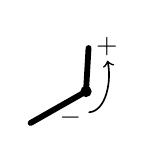
\begin{tikzpicture}[x=.8cm,y=.8cm,line cap=round,line join=round]
\draw[line width=2.1pt] (-.88,-.50)--(0,0)--(.04,.69);
\fill (0,0) circle[radius=.09];
\draw[->,line width=.6pt] (.05,-.33) .. controls (.32,-.31) and (.41,.17) .. (.34,.49);
\node at (.33,.72) {$+$}; \node at (-.25,-.41) {$-$};
\end{tikzpicture}}
l'arête ``origine'' et l'arête extrémité autour de $s$
% archive sheet number: 20
